\documentclass[10pt]{article}
\usepackage{itcep, stmaryrd, tikz, pgflibraryplotmarks, multicol}
\usepackage[margin=1in, nohead, pdftex]{geometry}
\usepackage{MnSymbol,wasysym}
\usepackage{hyperref}
\usepackage{enumitem}

\topmargin -0.2in
\pagestyle{empty}
\singlespacing
\let\oldhat\hat
\renewcommand{\vec}[1]{\mathbf{#1}}
\renewcommand{\hat}[1]{\oldhat{\mathbf{#1}}}

\definecolor{light-gray}{gray}{0.95}
\newcommand{\code}[1]{\colorbox{light-gray}{\texttt{#1}}}

\newcommand{\headerclass}{Machine Learning Camp}
\newcommand{\headersection}{Day 2: Exploring Data with Algorithms}
\newcommand{\headertitle}{Separating Hyperplanes}

\def\C{\mathbb{C}}
\def\R{\mathbb{R}}
\parindent 0ex
\begin{document}
%==================================================================================================================================================
\headerclass\xspace \hspace{\stretch{1}} \headersection\\
\begin{center}{ \large \textbf{\headertitle} }\end{center}
%==================================================================================================================================================

We'll soon introduce a new type of classifier, called a \emph{support vector machine}. We'll focus on \emph{linear} support vector machines, in particular a \emph{maximal margin classifier}.\\

The big idea is to pick a line so that all of the data from one class is on one side of the line, and all of the data from the other class is on the other side of the line. We also want to do this in the way that creates the most separation.\\

Let's see how this works for some fake data. Draw a line to separate the two groups plotted below.
\begin{center}
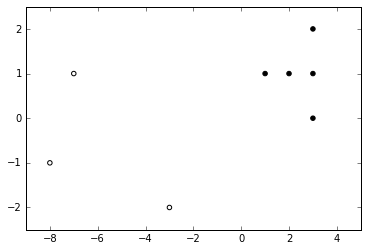
\includegraphics[scale = .75]{TwoClusters.png}
\end{center}
Compare the line you drew with the lines your neighbors drew. Do you have the same line? How did you decide what line to draw?\\

Discuss the following questions with your neighbors.

\begin{enumerate}
\item If I removed the white point at (-8,-1), would you change your separating line?
\vfill
\item If I removed the black point at (3,2), would you change your separating line?
\vfill
\item If I removed the white point at (-7,1), would you change your separating line?
\vfill
\item If I removed the black point at (3,0), would you change your separating line?
\vfill
\item Given your answers to the above, which points do you think matter the most?
\vfill
\end{enumerate}
The points that matter the most are called the \textit{support vectors}.

\newpage

In order to describe our dividing line, we'll use a linear function, something like $f(x_1,x_2) = 3x_1+2x_2-1$. The dividing line should be the set of points $(x_1,x_2)$ such that $f(x_1,x_2)=0$. Then the two sides of the line are where $f(x_1,x_2) >0$ and where $f(x_1,x_2) < 0$.\\

Let's see how this works for our fake data.

\begin{enumerate}[resume]
\item Write down the equation of your line in $y=mx+b$ form.
\vfill
\end{enumerate}

Now, we'll find our function $f(x_1,x_2)$.

\begin{enumerate}[resume]
\item Change your $x$ to $x_1$, and change your $y$ to $x_2$.
\vfill
\item Subtract everything over the right side of the equation, so the left side is just $0$.
\vfill
\item The function $f$ is defined by the right side of the equation above. Write 
\[f(x_1,x_2 ) = \underline{\hspace{2in}}\].
\item Plug in a few points to your new equation: if you plug in coordinates for white dots, do you get positive or negative numbers? If you plug in coordinates for black dots, do you get positive or negative numbers?
\vfill
\end{enumerate}

If all the white dots give you outputs with the same sign from $f(x_1,x_2)$, and all the black dots give you outputs with the opposite sign, you have made your first \textit{separating hyperplane}.\\

We'll use this idea of separating hyperplane to create a classifier called a support vector machine, which probably seems like a strange term to use. Let's break it down. 
\begin{itemize}
\item The support of a function is the set where the function isn't zero. Here it's really about where our function $f$ is positive and where it is negative, since that determines the classes.
\item More specifically, the support vectors are the training data points which are closest to the separating hyperplane. We saw that these points were most important. In this context, a vector is the same as a point: it has coordinates. A two-dimensional vector $\vec{x}$ is written $(x,y)$ or $(x_1, x_2)$, for instance. In other contexts, we might think of a vector as an arrow that points to a point, so it has a direction and a magnitude.
\item Machine: it sounds cool! Also, a machine is something designed to accomplish some task. Here, the task is classifying our data points.
\end{itemize}



\end{document}
